\documentclass{article}
\usepackage[paperwidth=841mm,paperheight=1189mm,margin=0mm]{geometry}
\usepackage[T1]{fontenc}
\usepackage[utf8]{inputenc}
\usepackage{lmodern,microtype,amsmath,amssymb,tikz,xcolor}
\usetikzlibrary{arrows.meta,calc,decorations.pathreplacing,positioning,shapes.geometric}
\pagestyle{empty}
\setlength{\parindent}{0pt}
\definecolor{ink}{gray}{0.03}
\definecolor{darkgray}{gray}{0.24}
\definecolor{midgray}{gray}{0.56}
\definecolor{softgray}{gray}{0.92}
\definecolor{panelgray}{gray}{0.965}
\definecolor{white}{gray}{1.00}
\pagecolor{white}
\color{ink}

\begin{document}
\begin{tikzpicture}[remember picture,overlay,x=1mm,y=1mm,
  >={Latex[length=6mm,width=4mm]},
  flow/.style={-Latex,line width=2.4pt,draw=ink},
  thinflow/.style={-Latex,line width=1.8pt,draw=ink},
  card/.style={draw=ink,fill=white,line width=1.8pt,rounded corners=8mm},
  labelbox/.style={fill=softgray,rounded corners=4mm},
  body/.style={font=\sffamily\fontsize{26}{33}\selectfont,text=ink},
  smallbody/.style={font=\sffamily\fontsize{22}{28}\selectfont,text=ink},
  heading/.style={font=\rmfamily\bfseries\fontsize{38}{43}\selectfont,text=ink}]
\begin{scope}[shift={(current page.south west)}]

% Title
\node[anchor=north,align=center,font=\rmfamily\bfseries\fontsize{86}{90}\selectfont]
  at (420.5,1176) {Refinement vs. Refresh};
\node[anchor=north,align=center,font=\rmfamily\fontsize{48}{54}\selectfont]
  at (420.5,1099) {Compute Allocation for Closed-Loop Robot Policies};
\draw[line width=1.6pt] (32,1057)--(168,1057);
\draw[line width=1.6pt] (673,1057)--(809,1057);
\node[anchor=center,align=center,font=\sffamily\fontsize{28}{34}\selectfont]
  at (420.5,1057) {Alba Mar\'ia T\'ellez Fern\'andez, MAAT Institute (alba.tellez@maatinstitute.com)};

% Closed-loop policy panel
\draw[card] (12,675) rectangle (829,1028);
\fill[softgray,rounded corners=8mm] (12,982) rectangle (286,1028);
\fill[softgray] (278,982)--(329,1028)--(278,1028)--cycle;
\node[anchor=west,heading] at (30,1004) {Chunked Closed-Loop Policy};

% Supplied closed-loop execution diagram
\node[anchor=center] at (420.5,850)
  {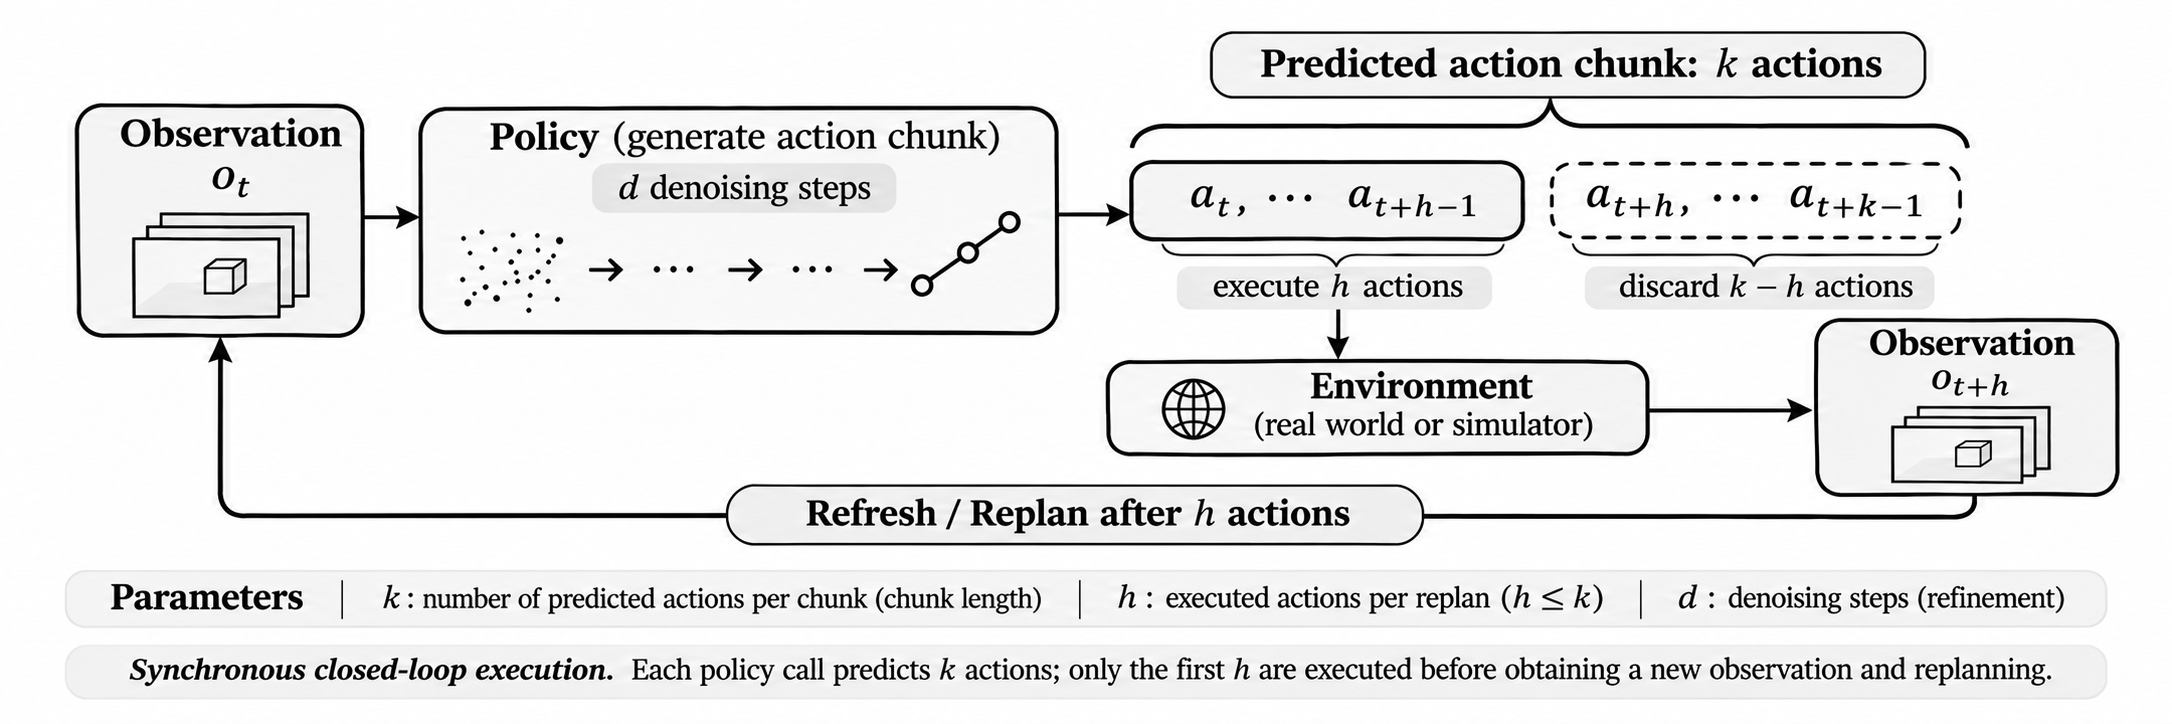
\includegraphics[width=780mm]{paper/figures/closed_loop_policy_diagram.png}};

% Central research question
\fill[softgray] (36,596) circle (25mm);
\node[font=\rmfamily\bfseries\fontsize{52}{56}\selectfont] at (36,596) {?};
\draw[line width=1.5pt] (76,561)--(76,630);
\node[anchor=west,align=left,text width=720mm,font=\rmfamily\fontsize{31}{39}\selectfont]
  at (96,596) {Under a fixed inference budget, should we allocate compute to additional denoising steps
  (\textbf{refinement}) or to more frequent observation-conditioned replanning (\textbf{refresh})?};

% Result card 1
\draw[card] (10,297) rectangle (411,533);
\fill[softgray,rounded corners=8mm] (10,495) rectangle (411,533);
\node[anchor=west,font=\rmfamily\bfseries\fontsize{32}{37}\selectfont]
  at (25,513) {Why the Trade-Off Exists};
\node[anchor=center] at (210.5,395)
  {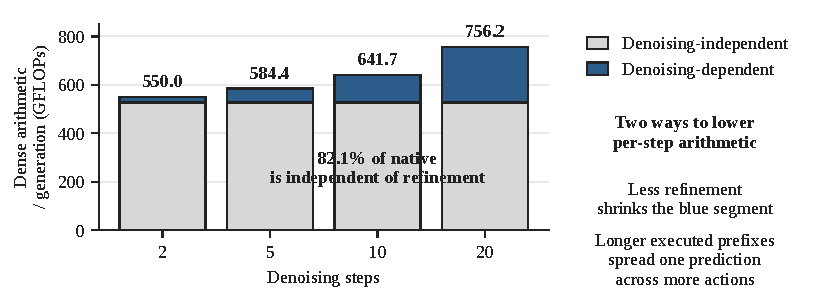
\includegraphics[width=390mm]{paper/generated/cost_decomposition.pdf}};

% Result card 2
\draw[card] (430,297) rectangle (831,533);
\fill[softgray,rounded corners=8mm] (430,495) rectangle (831,533);
\node[anchor=west,font=\rmfamily\bfseries\fontsize{32}{37}\selectfont]
  at (444,513) {Held-Out Success and Compute};
\node[anchor=center] at (630.5,395)
  {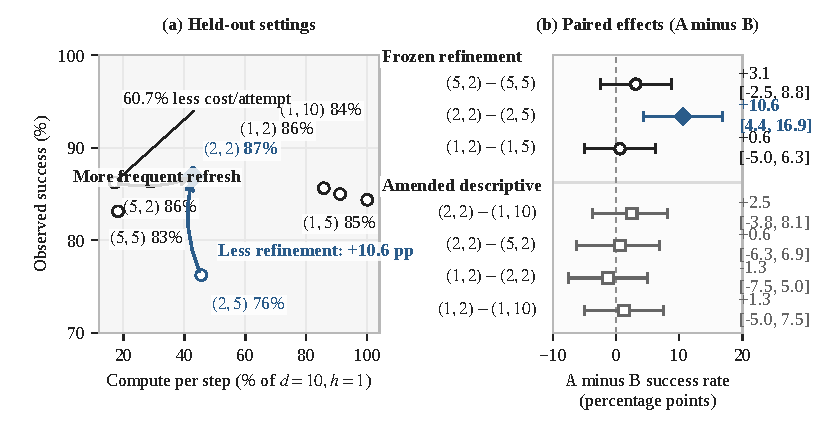
\includegraphics[width=385mm]{paper/generated/success_compute_tradeoff.pdf}};

% Compact interpretation
\draw[card] (10,24) rectangle (831,275);
\node[font=\rmfamily\bfseries\fontsize{35}{40}\selectfont] at (420.5,245)
  {A Recipe for Closed-Loop Compute Studies};
\draw[line width=1.4pt] (420.5,48)--(420.5,219);
\node[anchor=west,font=\rmfamily\bfseries\fontsize{29}{34}\selectfont] at (30,209)
  {Evaluate allocations within each model};
\node[anchor=north west,align=left,text width=360mm,font=\rmfamily\fontsize{25}{32}\selectfont]
  at (30,194) {1. Define refinement and refresh controls.\\2. Measure the complete cost of a fresh prediction.\\3. Freeze primary comparisons before held-out evaluation.\\4. Report success and expenditure together.};
\node[anchor=west,font=\rmfamily\bfseries\fontsize{29}{34}\selectfont] at (445,209)
  {Interpretation boundary};
\node[anchor=north west,align=left,text width=350mm,font=\rmfamily\fontsize{25}{32}\selectfont]
  at (445,194) {SmolVLA is the worked example, not a universal allocation rule. Arithmetic is not deployment latency, and similar observed success does not establish equivalent quality.};

\end{scope}
\end{tikzpicture}
\end{document}
